% Options for packages loaded elsewhere
\PassOptionsToPackage{unicode}{hyperref}
\PassOptionsToPackage{hyphens}{url}
%
\documentclass[
]{article}
\usepackage{amsmath,amssymb}
\usepackage{lmodern}
\usepackage{iftex}
\ifPDFTeX
  \usepackage[T1]{fontenc}
  \usepackage[utf8]{inputenc}
  \usepackage{textcomp} % provide euro and other symbols
\else % if luatex or xetex
  \usepackage{unicode-math}
  \defaultfontfeatures{Scale=MatchLowercase}
  \defaultfontfeatures[\rmfamily]{Ligatures=TeX,Scale=1}
\fi
% Use upquote if available, for straight quotes in verbatim environments
\IfFileExists{upquote.sty}{\usepackage{upquote}}{}
\IfFileExists{microtype.sty}{% use microtype if available
  \usepackage[]{microtype}
  \UseMicrotypeSet[protrusion]{basicmath} % disable protrusion for tt fonts
}{}
\makeatletter
\@ifundefined{KOMAClassName}{% if non-KOMA class
  \IfFileExists{parskip.sty}{%
    \usepackage{parskip}
  }{% else
    \setlength{\parindent}{0pt}
    \setlength{\parskip}{6pt plus 2pt minus 1pt}}
}{% if KOMA class
  \KOMAoptions{parskip=half}}
\makeatother
\usepackage{xcolor}
\usepackage[margin=1in]{geometry}
\usepackage{color}
\usepackage{fancyvrb}
\newcommand{\VerbBar}{|}
\newcommand{\VERB}{\Verb[commandchars=\\\{\}]}
\DefineVerbatimEnvironment{Highlighting}{Verbatim}{commandchars=\\\{\}}
% Add ',fontsize=\small' for more characters per line
\usepackage{framed}
\definecolor{shadecolor}{RGB}{248,248,248}
\newenvironment{Shaded}{\begin{snugshade}}{\end{snugshade}}
\newcommand{\AlertTok}[1]{\textcolor[rgb]{0.94,0.16,0.16}{#1}}
\newcommand{\AnnotationTok}[1]{\textcolor[rgb]{0.56,0.35,0.01}{\textbf{\textit{#1}}}}
\newcommand{\AttributeTok}[1]{\textcolor[rgb]{0.77,0.63,0.00}{#1}}
\newcommand{\BaseNTok}[1]{\textcolor[rgb]{0.00,0.00,0.81}{#1}}
\newcommand{\BuiltInTok}[1]{#1}
\newcommand{\CharTok}[1]{\textcolor[rgb]{0.31,0.60,0.02}{#1}}
\newcommand{\CommentTok}[1]{\textcolor[rgb]{0.56,0.35,0.01}{\textit{#1}}}
\newcommand{\CommentVarTok}[1]{\textcolor[rgb]{0.56,0.35,0.01}{\textbf{\textit{#1}}}}
\newcommand{\ConstantTok}[1]{\textcolor[rgb]{0.00,0.00,0.00}{#1}}
\newcommand{\ControlFlowTok}[1]{\textcolor[rgb]{0.13,0.29,0.53}{\textbf{#1}}}
\newcommand{\DataTypeTok}[1]{\textcolor[rgb]{0.13,0.29,0.53}{#1}}
\newcommand{\DecValTok}[1]{\textcolor[rgb]{0.00,0.00,0.81}{#1}}
\newcommand{\DocumentationTok}[1]{\textcolor[rgb]{0.56,0.35,0.01}{\textbf{\textit{#1}}}}
\newcommand{\ErrorTok}[1]{\textcolor[rgb]{0.64,0.00,0.00}{\textbf{#1}}}
\newcommand{\ExtensionTok}[1]{#1}
\newcommand{\FloatTok}[1]{\textcolor[rgb]{0.00,0.00,0.81}{#1}}
\newcommand{\FunctionTok}[1]{\textcolor[rgb]{0.00,0.00,0.00}{#1}}
\newcommand{\ImportTok}[1]{#1}
\newcommand{\InformationTok}[1]{\textcolor[rgb]{0.56,0.35,0.01}{\textbf{\textit{#1}}}}
\newcommand{\KeywordTok}[1]{\textcolor[rgb]{0.13,0.29,0.53}{\textbf{#1}}}
\newcommand{\NormalTok}[1]{#1}
\newcommand{\OperatorTok}[1]{\textcolor[rgb]{0.81,0.36,0.00}{\textbf{#1}}}
\newcommand{\OtherTok}[1]{\textcolor[rgb]{0.56,0.35,0.01}{#1}}
\newcommand{\PreprocessorTok}[1]{\textcolor[rgb]{0.56,0.35,0.01}{\textit{#1}}}
\newcommand{\RegionMarkerTok}[1]{#1}
\newcommand{\SpecialCharTok}[1]{\textcolor[rgb]{0.00,0.00,0.00}{#1}}
\newcommand{\SpecialStringTok}[1]{\textcolor[rgb]{0.31,0.60,0.02}{#1}}
\newcommand{\StringTok}[1]{\textcolor[rgb]{0.31,0.60,0.02}{#1}}
\newcommand{\VariableTok}[1]{\textcolor[rgb]{0.00,0.00,0.00}{#1}}
\newcommand{\VerbatimStringTok}[1]{\textcolor[rgb]{0.31,0.60,0.02}{#1}}
\newcommand{\WarningTok}[1]{\textcolor[rgb]{0.56,0.35,0.01}{\textbf{\textit{#1}}}}
\usepackage{graphicx}
\makeatletter
\def\maxwidth{\ifdim\Gin@nat@width>\linewidth\linewidth\else\Gin@nat@width\fi}
\def\maxheight{\ifdim\Gin@nat@height>\textheight\textheight\else\Gin@nat@height\fi}
\makeatother
% Scale images if necessary, so that they will not overflow the page
% margins by default, and it is still possible to overwrite the defaults
% using explicit options in \includegraphics[width, height, ...]{}
\setkeys{Gin}{width=\maxwidth,height=\maxheight,keepaspectratio}
% Set default figure placement to htbp
\makeatletter
\def\fps@figure{htbp}
\makeatother
\setlength{\emergencystretch}{3em} % prevent overfull lines
\providecommand{\tightlist}{%
  \setlength{\itemsep}{0pt}\setlength{\parskip}{0pt}}
\setcounter{secnumdepth}{-\maxdimen} % remove section numbering
\ifLuaTeX
  \usepackage{selnolig}  % disable illegal ligatures
\fi
\IfFileExists{bookmark.sty}{\usepackage{bookmark}}{\usepackage{hyperref}}
\IfFileExists{xurl.sty}{\usepackage{xurl}}{} % add URL line breaks if available
\urlstyle{same} % disable monospaced font for URLs
\hypersetup{
  pdftitle={V1075 Monte Carlo},
  pdfauthor={Matthew Allen},
  hidelinks,
  pdfcreator={LaTeX via pandoc}}

\title{V1075 Monte Carlo}
\author{Matthew Allen}
\date{December 2023}

\begin{document}
\maketitle

\hypertarget{step-1-load-packages-and-data}{%
\subsection{Step 1: Load packages and
data}\label{step-1-load-packages-and-data}}

\hypertarget{i-want-to-source-the-data-directly-from-github-but-rmarkdown-is-giving-me-trouble}{%
\subsection{!!! I want to source the data directly from GitHub, but
Rmarkdown is giving me trouble
!!!}\label{i-want-to-source-the-data-directly-from-github-but-rmarkdown-is-giving-me-trouble}}

\begin{Shaded}
\begin{Highlighting}[]
\CommentTok{\# Load required packages}
\FunctionTok{library}\NormalTok{(dplyr)}
\FunctionTok{library}\NormalTok{(purrr)}
\FunctionTok{library}\NormalTok{(ggplot2)}
\FunctionTok{library}\NormalTok{(RCurl)}

\CommentTok{\# !!! V1075\_MCdata is sourced from script "V1075\_d18O\_wrangle.R"}

\CommentTok{\# local, if needed}
  \FunctionTok{setwd}\NormalTok{(}\StringTok{"/Users/allen/Documents/GitHub/1075\_Vertebrate\_d18Op/Data"}\NormalTok{)}
\NormalTok{  V1075\_MCdata }\OtherTok{\textless{}{-}} \FunctionTok{read.csv}\NormalTok{(}\StringTok{"V1075MC\_data.csv"}\NormalTok{)}
\NormalTok{  NIST120c }\OtherTok{\textless{}{-}} \FunctionTok{read.csv}\NormalTok{(}\StringTok{"V1075\_NIST120c.csv"}\NormalTok{)}

\CommentTok{\# Set number of Monte Carlo repetitions }
\NormalTok{nMCrepetitions }\OtherTok{\textless{}{-}} \FloatTok{1e3}

\CommentTok{\# Subset V1075\_cl by biological group}
\NormalTok{gar }\OtherTok{\textless{}{-}} \FunctionTok{subset}\NormalTok{(V1075\_MCdata, Taxon }\SpecialCharTok{==} \StringTok{"Lepisosteids"}\NormalTok{)}
\NormalTok{shark }\OtherTok{\textless{}{-}} \FunctionTok{subset}\NormalTok{(V1075\_MCdata, Taxon }\SpecialCharTok{==} \StringTok{"Hybodonts"}\NormalTok{)}
\NormalTok{glyptops }\OtherTok{\textless{}{-}} \FunctionTok{subset}\NormalTok{(V1075\_MCdata, Taxon }\SpecialCharTok{==} \StringTok{"Glyptops sp."}\NormalTok{)}
\NormalTok{naomichelys }\OtherTok{\textless{}{-}} \FunctionTok{subset}\NormalTok{(V1075\_MCdata, Taxon }\SpecialCharTok{==} \StringTok{"Naomichelys sp."}\NormalTok{)}
\NormalTok{crocG }\OtherTok{\textless{}{-}} \FunctionTok{subset}\NormalTok{(V1075\_MCdata, Taxon }\SpecialCharTok{==} \StringTok{"Neosuchian G"}\NormalTok{)}
\NormalTok{crocA }\OtherTok{\textless{}{-}} \FunctionTok{subset}\NormalTok{(V1075\_MCdata, Taxon }\SpecialCharTok{==} \StringTok{"Neosuchian A"}\NormalTok{)}
\NormalTok{crocB }\OtherTok{\textless{}{-}} \FunctionTok{subset}\NormalTok{(V1075\_MCdata, Taxon }\SpecialCharTok{==} \StringTok{"Neosuchian B"}\NormalTok{)}

\CommentTok{\# Bootstrapping}
\CommentTok{\# Resample d18Op for each taxon}
\CommentTok{\# Take mean of each resample}
\CommentTok{\# Compile means in data frame}

\NormalTok{synth\_shark }\OtherTok{\textless{}{-}} \FunctionTok{data\_frame}\NormalTok{(}\AttributeTok{num =} \DecValTok{1}\SpecialCharTok{:}\NormalTok{nMCrepetitions) }\SpecialCharTok{\%\textgreater{}\%} 
  \FunctionTok{group\_by}\NormalTok{(num) }\SpecialCharTok{\%\textgreater{}\%} 
  \FunctionTok{mutate}\NormalTok{(}\AttributeTok{means =} \FunctionTok{mean}\NormalTok{(}\FunctionTok{sample}\NormalTok{(shark}\SpecialCharTok{$}\NormalTok{d18O, }\AttributeTok{replace =} \ConstantTok{TRUE}\NormalTok{))) }

\NormalTok{synth\_gar }\OtherTok{\textless{}{-}} \FunctionTok{data\_frame}\NormalTok{(}\AttributeTok{num =} \DecValTok{1}\SpecialCharTok{:}\NormalTok{nMCrepetitions) }\SpecialCharTok{\%\textgreater{}\%} 
  \FunctionTok{group\_by}\NormalTok{(num) }\SpecialCharTok{\%\textgreater{}\%} 
  \FunctionTok{mutate}\NormalTok{(}\AttributeTok{means =} \FunctionTok{mean}\NormalTok{(}\FunctionTok{sample}\NormalTok{(gar}\SpecialCharTok{$}\NormalTok{d18O, }\AttributeTok{replace =} \ConstantTok{TRUE}\NormalTok{))) }
\FunctionTok{mean}\NormalTok{(synth\_gar}\SpecialCharTok{$}\NormalTok{means)}

\NormalTok{synth\_glyptops }\OtherTok{\textless{}{-}} \FunctionTok{data\_frame}\NormalTok{(}\AttributeTok{num =} \DecValTok{1}\SpecialCharTok{:}\NormalTok{nMCrepetitions) }\SpecialCharTok{\%\textgreater{}\%} 
  \FunctionTok{group\_by}\NormalTok{(num) }\SpecialCharTok{\%\textgreater{}\%} 
  \FunctionTok{mutate}\NormalTok{(}\AttributeTok{means =} \FunctionTok{mean}\NormalTok{(}\FunctionTok{sample}\NormalTok{(glyptops}\SpecialCharTok{$}\NormalTok{d18O, }\AttributeTok{replace =} \ConstantTok{TRUE}\NormalTok{))) }

\NormalTok{synth\_naomichelys }\OtherTok{\textless{}{-}} \FunctionTok{data\_frame}\NormalTok{(}\AttributeTok{num =} \DecValTok{1}\SpecialCharTok{:}\NormalTok{nMCrepetitions) }\SpecialCharTok{\%\textgreater{}\%} 
  \FunctionTok{group\_by}\NormalTok{(num) }\SpecialCharTok{\%\textgreater{}\%} 
  \FunctionTok{mutate}\NormalTok{(}\AttributeTok{means =} \FunctionTok{mean}\NormalTok{(}\FunctionTok{sample}\NormalTok{(naomichelys}\SpecialCharTok{$}\NormalTok{d18O, }\AttributeTok{replace =} \ConstantTok{TRUE}\NormalTok{))) }

\NormalTok{synth\_crocG }\OtherTok{\textless{}{-}} \FunctionTok{data\_frame}\NormalTok{(}\AttributeTok{num =} \DecValTok{1}\SpecialCharTok{:}\NormalTok{nMCrepetitions) }\SpecialCharTok{\%\textgreater{}\%} 
  \FunctionTok{group\_by}\NormalTok{(num) }\SpecialCharTok{\%\textgreater{}\%} 
  \FunctionTok{mutate}\NormalTok{(}\AttributeTok{means =} \FunctionTok{mean}\NormalTok{(}\FunctionTok{sample}\NormalTok{(crocG}\SpecialCharTok{$}\NormalTok{d18O, }\AttributeTok{replace =} \ConstantTok{TRUE}\NormalTok{))) }

\NormalTok{synth\_crocA }\OtherTok{\textless{}{-}} \FunctionTok{data\_frame}\NormalTok{(}\AttributeTok{num =} \DecValTok{1}\SpecialCharTok{:}\NormalTok{nMCrepetitions) }\SpecialCharTok{\%\textgreater{}\%} 
  \FunctionTok{group\_by}\NormalTok{(num) }\SpecialCharTok{\%\textgreater{}\%} 
  \FunctionTok{mutate}\NormalTok{(}\AttributeTok{means =} \FunctionTok{mean}\NormalTok{(}\FunctionTok{sample}\NormalTok{(crocA}\SpecialCharTok{$}\NormalTok{d18O, }\AttributeTok{replace =} \ConstantTok{TRUE}\NormalTok{))) }

\NormalTok{synth\_crocB }\OtherTok{\textless{}{-}} \FunctionTok{data\_frame}\NormalTok{(}\AttributeTok{num =} \DecValTok{1}\SpecialCharTok{:}\NormalTok{nMCrepetitions) }\SpecialCharTok{\%\textgreater{}\%} 
  \FunctionTok{group\_by}\NormalTok{(num) }\SpecialCharTok{\%\textgreater{}\%} 
  \FunctionTok{mutate}\NormalTok{(}\AttributeTok{means =} \FunctionTok{mean}\NormalTok{(}\FunctionTok{sample}\NormalTok{(crocB}\SpecialCharTok{$}\NormalTok{d18O, }\AttributeTok{replace =} \ConstantTok{TRUE}\NormalTok{))) }

\NormalTok{synth\_NIST }\OtherTok{\textless{}{-}} \FunctionTok{data\_frame}\NormalTok{(}\AttributeTok{num =} \DecValTok{1}\SpecialCharTok{:}\NormalTok{nMCrepetitions) }\SpecialCharTok{\%\textgreater{}\%} 
  \FunctionTok{group\_by}\NormalTok{(num) }\SpecialCharTok{\%\textgreater{}\%} 
  \FunctionTok{mutate}\NormalTok{(}\AttributeTok{means =} \FunctionTok{mean}\NormalTok{(}\FunctionTok{sample}\NormalTok{(NIST120c}\SpecialCharTok{$}\NormalTok{d}\FloatTok{.18}\NormalTok{O}\FloatTok{.16}\NormalTok{O, }\AttributeTok{replace =} \ConstantTok{TRUE}\NormalTok{))) }

\CommentTok{\# Combine data frames into one}
\NormalTok{combined\_data }\OtherTok{\textless{}{-}} \FunctionTok{rbind}\NormalTok{(}
  \FunctionTok{data.frame}\NormalTok{(}\AttributeTok{group =} \StringTok{"Gar"}\NormalTok{, }\AttributeTok{values =}\NormalTok{ synth\_gar}\SpecialCharTok{$}\NormalTok{means),}
  \FunctionTok{data.frame}\NormalTok{(}\AttributeTok{group =} \StringTok{"Sharks"}\NormalTok{, }\AttributeTok{values =}\NormalTok{ synth\_shark}\SpecialCharTok{$}\NormalTok{means),}
  \FunctionTok{data.frame}\NormalTok{(}\AttributeTok{group =} \StringTok{"Glyptops"}\NormalTok{, }\AttributeTok{values =}\NormalTok{ synth\_glyptops}\SpecialCharTok{$}\NormalTok{means),}
  \FunctionTok{data.frame}\NormalTok{(}\AttributeTok{group =} \StringTok{"Naomichelys"}\NormalTok{, }\AttributeTok{values =}\NormalTok{ synth\_naomichelys}\SpecialCharTok{$}\NormalTok{means),}
  \FunctionTok{data.frame}\NormalTok{(}\AttributeTok{group =} \StringTok{"Neosuchian G"}\NormalTok{, }\AttributeTok{values =}\NormalTok{ synth\_crocG}\SpecialCharTok{$}\NormalTok{means),}
  \FunctionTok{data.frame}\NormalTok{(}\AttributeTok{group =} \StringTok{"Neosuchian A"}\NormalTok{, }\AttributeTok{values =}\NormalTok{ synth\_crocA}\SpecialCharTok{$}\NormalTok{means),}
  \FunctionTok{data.frame}\NormalTok{(}\AttributeTok{group =} \StringTok{"Neosuchian B"}\NormalTok{, }\AttributeTok{values =}\NormalTok{ synth\_crocB}\SpecialCharTok{$}\NormalTok{means),}
  \FunctionTok{data.frame}\NormalTok{(}\AttributeTok{group =} \StringTok{"NIST"}\NormalTok{, }\AttributeTok{values =}\NormalTok{ synth\_NIST}\SpecialCharTok{$}\NormalTok{means)}
\NormalTok{)}

\CommentTok{\# Set order of facets}
\NormalTok{combined\_data}\SpecialCharTok{$}\NormalTok{group }\OtherTok{\textless{}{-}} \FunctionTok{factor}\NormalTok{(combined\_data}\SpecialCharTok{$}\NormalTok{group, }\AttributeTok{levels =} \FunctionTok{c}\NormalTok{(}\StringTok{"Gar"}\NormalTok{, }\StringTok{"Sharks"}\NormalTok{, }\StringTok{"Glyptops"}\NormalTok{, }\StringTok{"Neosuchian G"}\NormalTok{, }\StringTok{"Neosuchian A"}\NormalTok{, }\StringTok{"Neosuchian B"}\NormalTok{, }\StringTok{"Naomichelys"}\NormalTok{, }\StringTok{"NIST"}\NormalTok{))}

\CommentTok{\# Plot histogram of resampled means for each taxon}
\FunctionTok{ggplot}\NormalTok{(combined\_data, }\FunctionTok{aes}\NormalTok{(}\AttributeTok{x =}\NormalTok{ values, }\AttributeTok{fill =}\NormalTok{ group)) }\SpecialCharTok{+}
  \FunctionTok{geom\_histogram}\NormalTok{(}\AttributeTok{position =} \StringTok{"identity"}\NormalTok{, }\AttributeTok{alpha =} \FloatTok{0.7}\NormalTok{, }\AttributeTok{bins =} \DecValTok{30}\NormalTok{, }\AttributeTok{color =} \StringTok{"black"}\NormalTok{) }\SpecialCharTok{+}
  \FunctionTok{labs}\NormalTok{(}\AttributeTok{title =} \StringTok{"Histogram of Means"}\NormalTok{,}
       \AttributeTok{x =} \StringTok{"Means"}\NormalTok{,}
       \AttributeTok{y =} \StringTok{"Frequency"}\NormalTok{) }\SpecialCharTok{+}
  \FunctionTok{theme\_minimal}\NormalTok{() }\SpecialCharTok{+}
  \FunctionTok{facet\_wrap}\NormalTok{(}\SpecialCharTok{\textasciitilde{}}\NormalTok{group, }\AttributeTok{scales =} \StringTok{"free"}\NormalTok{)}
\end{Highlighting}
\end{Shaded}

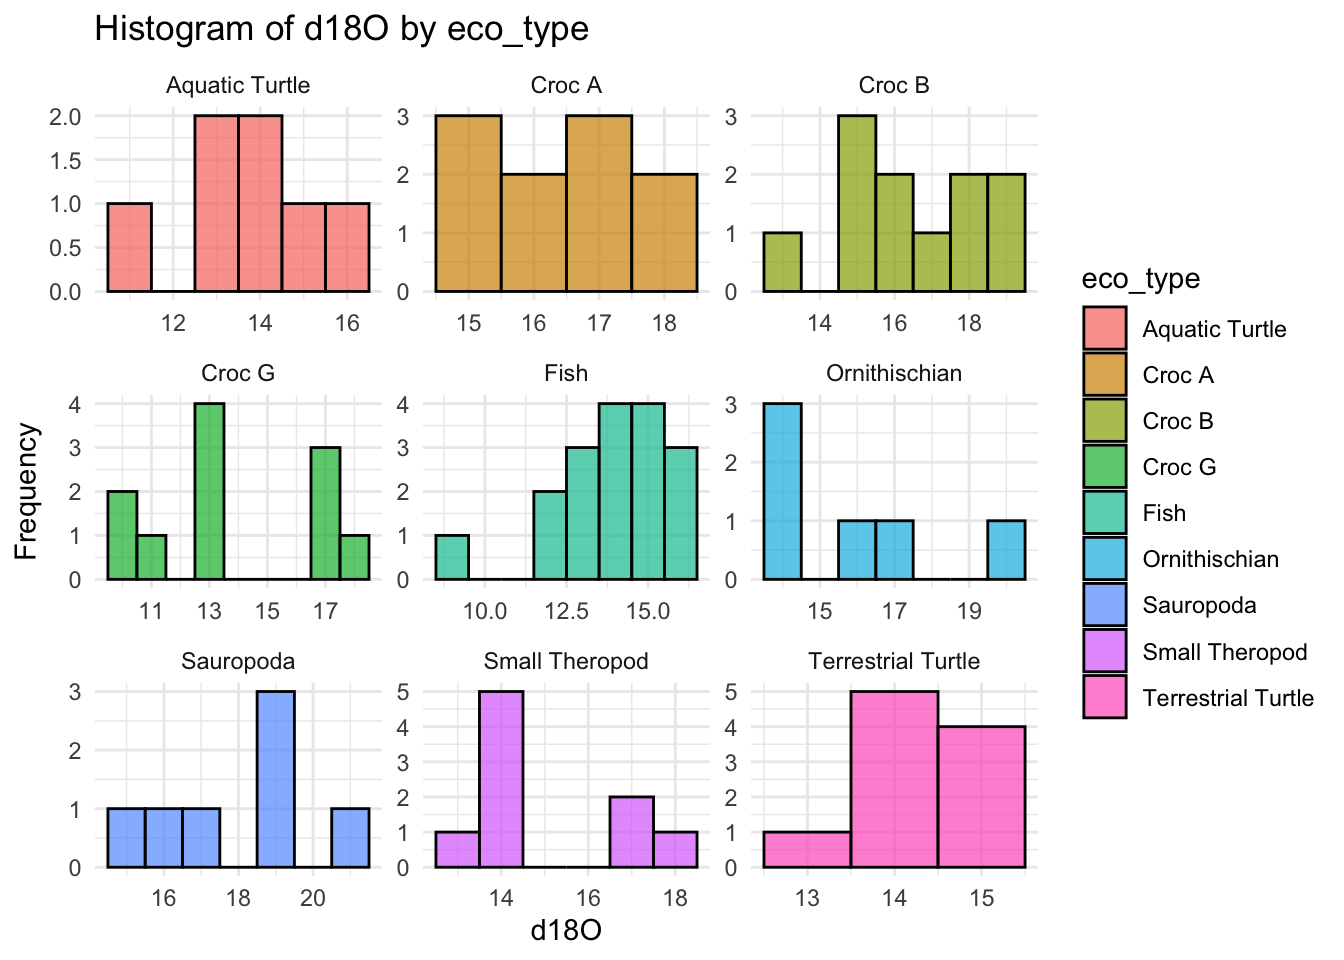
\includegraphics{V1075_MonteCarlo_files/figure-latex/unnamed-chunk-1-1.pdf}

\begin{Shaded}
\begin{Highlighting}[]
\CommentTok{\# Load the regression models}

\CommentTok{\# Load Barrick regression model (from \textasciitilde{}/Documents/GitHub/1075\_Vertebrate\_d18Op/Code/d18Ow\_Proxy\_Regressions.R)}
\NormalTok{Barrick\_lm\_model }\OtherTok{\textless{}{-}} \FunctionTok{readRDS}\NormalTok{(}\StringTok{"/Users/allen/Documents/GitHub/1075\_Vertebrate\_d18Op/Data/Barrick\_reg\_lm.rds"}\NormalTok{)}

\CommentTok{\# Load Amiot regression model (from \textasciitilde{}/Documents/GitHub/1075\_Vertebrate\_d18Op/Code/d18Ow\_Proxy\_Regressions.R)}
\NormalTok{Amiot\_lm\_model }\OtherTok{\textless{}{-}} \FunctionTok{readRDS}\NormalTok{(}\StringTok{"/Users/allen/Documents/GitHub/1075\_Vertebrate\_d18Op/Data/Amiot\_reg\_lm.rds"}\NormalTok{)}

\CommentTok{\# Load Puceat, Longinelli, Nuti (PLN) regression model (from \textasciitilde{}/Documents/GitHub/1075\_Vertebrate\_d18Op/Code/d18Ow\_Proxy\_Regressions.R)}
\NormalTok{PLN\_lm\_model }\OtherTok{\textless{}{-}} \FunctionTok{readRDS}\NormalTok{(}\StringTok{"/Users/allen/Documents/GitHub/1075\_Vertebrate\_d18Op/Data/PLNd18Op\_reg\_lm.rds"}\NormalTok{)}

\CommentTok{\# Load Tw\textasciitilde{}Ta transform model (from )}
\NormalTok{TwTa\_lm\_model }\OtherTok{\textless{}{-}} \FunctionTok{readRDS}\NormalTok{(}\StringTok{"/Users/allen/Documents/GitHub/1075\_Vertebrate\_d18Op/Data/TwTa\_reg\_lm.rds"}\NormalTok{)}


\FunctionTok{summary}\NormalTok{(Barrick\_lm\_model)}
\FunctionTok{summary}\NormalTok{(Amiot\_lm\_model)}
\FunctionTok{summary}\NormalTok{(PLN\_lm\_model)}
\end{Highlighting}
\end{Shaded}

\hypertarget{croc-water}{%
\section{Croc Water}\label{croc-water}}

\begin{Shaded}
\begin{Highlighting}[]
\CommentTok{\# Croc Water {-}{-}{-}{-}{-}{-}{-}{-}{-}{-}{-}{-}{-}{-}{-}{-}{-}{-}{-}{-}{-}{-}{-}{-}{-}{-}{-}{-}{-}{-}{-}{-}{-}{-}{-}{-}{-}{-}{-}{-}{-}{-}{-}{-}{-}{-}{-}{-}{-}{-}{-}{-}{-}{-}{-}{-}{-}{-}{-}{-}{-}{-}}

\CommentTok{\# Extract the regression coefficients and standard errors}
\NormalTok{Amiot\_model\_summary }\OtherTok{\textless{}{-}} \FunctionTok{summary}\NormalTok{(Amiot\_lm\_model)}
\NormalTok{Amiot\_intercept }\OtherTok{\textless{}{-}} \FunctionTok{coef}\NormalTok{(Amiot\_lm\_model)[}\DecValTok{1}\NormalTok{]}
\NormalTok{Amiot\_slope }\OtherTok{\textless{}{-}} \FunctionTok{coef}\NormalTok{(Amiot\_lm\_model)[}\DecValTok{2}\NormalTok{]}
\NormalTok{Amiot\_intercept\_se }\OtherTok{\textless{}{-}} \FunctionTok{coef}\NormalTok{(Amiot\_model\_summary)[}\DecValTok{1}\NormalTok{, }\StringTok{"Std. Error"}\NormalTok{]  }\CommentTok{\# Standard error for intercept}
\NormalTok{Amiot\_slope\_se }\OtherTok{\textless{}{-}} \FunctionTok{coef}\NormalTok{(Amiot\_model\_summary)[}\DecValTok{2}\NormalTok{, }\StringTok{"Std. Error"}\NormalTok{]      }\CommentTok{\# Standard error for slope}

\FunctionTok{cat}\NormalTok{(}\StringTok{"Standard Error for Intercept:"}\NormalTok{, Amiot\_intercept\_se, }\StringTok{"}\SpecialCharTok{\textbackslash{}n}\StringTok{"}\NormalTok{)}
\end{Highlighting}
\end{Shaded}

\begin{verbatim}
## Standard Error for Intercept: 1.076794
\end{verbatim}

\begin{Shaded}
\begin{Highlighting}[]
\FunctionTok{cat}\NormalTok{(}\StringTok{"Standard Error for Slope:"}\NormalTok{, Amiot\_slope\_se, }\StringTok{"}\SpecialCharTok{\textbackslash{}n}\StringTok{"}\NormalTok{)}
\end{Highlighting}
\end{Shaded}

\begin{verbatim}
## Standard Error for Slope: 0.06216893
\end{verbatim}

\begin{Shaded}
\begin{Highlighting}[]
\CommentTok{\# Simulate regression coefficients for the regression model}
\FunctionTok{set.seed}\NormalTok{(}\DecValTok{123}\NormalTok{)  }\CommentTok{\# For reproducibility}
\NormalTok{n\_iterations }\OtherTok{\textless{}{-}} \FloatTok{1e3}  \CommentTok{\# Number of Monte Carlo simulations}

\CommentTok{\# Define }
\NormalTok{Amiot\_residual\_sd }\OtherTok{\textless{}{-}} \FunctionTok{summary}\NormalTok{(Amiot\_lm\_model)}\SpecialCharTok{$}\NormalTok{sigma}

\CommentTok{\# Generate simulated slope and intercept values}
\NormalTok{Amiot\_simulated\_slope }\OtherTok{\textless{}{-}} \FunctionTok{rnorm}\NormalTok{(n\_iterations, }\AttributeTok{mean =}\NormalTok{ Amiot\_slope, }\AttributeTok{sd =}\NormalTok{ Amiot\_slope\_se)}
\NormalTok{Amiot\_simulated\_intercept }\OtherTok{\textless{}{-}} \FunctionTok{rnorm}\NormalTok{(n\_iterations, }\AttributeTok{mean =}\NormalTok{ Amiot\_intercept, }\AttributeTok{sd =}\NormalTok{ Amiot\_intercept\_se)}

\CommentTok{\# Monte Carlo simulation for the regression}
\CommentTok{\# simulate residual error}
\NormalTok{Amiot\_residual\_error }\OtherTok{\textless{}{-}} \FunctionTok{rnorm}\NormalTok{(n\_iterations, }\AttributeTok{mean =} \DecValTok{0}\NormalTok{, }\AttributeTok{sd =}\NormalTok{ Amiot\_residual\_sd)}

\CommentTok{\# Store Croc G d18Op synth means in vector}
\NormalTok{crocG\_synthmeans\_d18Op }\OtherTok{\textless{}{-}}\NormalTok{ synth\_crocG}\SpecialCharTok{$}\NormalTok{means}
\FunctionTok{mean}\NormalTok{(crocG\_synthmeans\_d18Op)}
\end{Highlighting}
\end{Shaded}

\begin{verbatim}
## [1] 14.07078
\end{verbatim}

\begin{Shaded}
\begin{Highlighting}[]
\CommentTok{\# Expand d18Op values to interact with all simulated parameters}
\NormalTok{expanded\_d18Op }\OtherTok{\textless{}{-}} \FunctionTok{rep}\NormalTok{(crocG\_synthmeans\_d18Op, }\AttributeTok{each =}\NormalTok{ n\_iterations)}
\NormalTok{expanded\_slopes }\OtherTok{\textless{}{-}} \FunctionTok{rep}\NormalTok{(Amiot\_simulated\_slope, }\AttributeTok{times =} \FunctionTok{length}\NormalTok{(crocG\_synthmeans\_d18Op))}
\NormalTok{expanded\_intercepts }\OtherTok{\textless{}{-}} \FunctionTok{rep}\NormalTok{(Amiot\_simulated\_intercept, }\AttributeTok{times =} \FunctionTok{length}\NormalTok{(crocG\_synthmeans\_d18Op))}
\NormalTok{expanded\_residuals }\OtherTok{\textless{}{-}} \FunctionTok{rep}\NormalTok{(Amiot\_residual\_error, }\AttributeTok{times =} \FunctionTok{length}\NormalTok{(crocG\_synthmeans\_d18Op))}

\CommentTok{\# Calculate water simulations}
\NormalTok{crocG\_water\_simulations }\OtherTok{\textless{}{-}}\NormalTok{ expanded\_slopes }\SpecialCharTok{*}\NormalTok{ expanded\_d18Op }\SpecialCharTok{+}\NormalTok{ expanded\_intercepts }\SpecialCharTok{+}\NormalTok{ expanded\_residuals}
\FunctionTok{mean}\NormalTok{(crocG\_water\_simulations)}
\end{Highlighting}
\end{Shaded}

\begin{verbatim}
## [1] -7.51277
\end{verbatim}

\begin{Shaded}
\begin{Highlighting}[]
\CommentTok{\# Sort the simulated water values}
\NormalTok{sorted\_crocG\_synthd18Owater }\OtherTok{\textless{}{-}} \FunctionTok{sort}\NormalTok{(crocG\_water\_simulations)}

\CommentTok{\# Calculate 95\% CI percentiles}
\NormalTok{crocwatersynth\_lower\_95\_CI }\OtherTok{\textless{}{-}} \FunctionTok{quantile}\NormalTok{(sorted\_crocG\_synthd18Owater, }\AttributeTok{probs =} \FloatTok{0.025}\NormalTok{)}
\NormalTok{crocwatersynth\_upper\_95\_CI }\OtherTok{\textless{}{-}} \FunctionTok{quantile}\NormalTok{(sorted\_crocG\_synthd18Owater, }\AttributeTok{probs =} \FloatTok{0.975}\NormalTok{)}

\CommentTok{\# Compute the mean of the data}
\NormalTok{mean\_crocwater\_synth }\OtherTok{\textless{}{-}} \FunctionTok{mean}\NormalTok{(sorted\_crocG\_synthd18Owater)}

\CommentTok{\# Print the results}
\FunctionTok{cat}\NormalTok{(}\StringTok{"Mean crocG d18Owater:"}\NormalTok{, }\FunctionTok{round}\NormalTok{(mean\_crocwater\_synth, }\DecValTok{2}\NormalTok{), }\StringTok{"}\SpecialCharTok{\textbackslash{}n}\StringTok{"}\NormalTok{)}
\end{Highlighting}
\end{Shaded}

\begin{verbatim}
## Mean crocG d18Owater: -7.51
\end{verbatim}

\begin{Shaded}
\begin{Highlighting}[]
\FunctionTok{cat}\NormalTok{(}\StringTok{"95\% CI for crocG d18Owater: ["}\NormalTok{, }\FunctionTok{round}\NormalTok{(crocwatersynth\_lower\_95\_CI, }\DecValTok{2}\NormalTok{), }\StringTok{","}\NormalTok{, }\FunctionTok{round}\NormalTok{(crocwatersynth\_upper\_95\_CI, }\DecValTok{2}\NormalTok{), }\StringTok{"]}\SpecialCharTok{\textbackslash{}n}\StringTok{"}\NormalTok{)}
\end{Highlighting}
\end{Shaded}

\begin{verbatim}
## 95% CI for crocG d18Owater: [ -11.16 , -3.56 ]
\end{verbatim}

\hypertarget{turtle-water}{%
\section{Turtle Water}\label{turtle-water}}

\begin{Shaded}
\begin{Highlighting}[]
\CommentTok{\# Extract the regression coefficients and standard errors}
\NormalTok{Barrick\_model\_summary }\OtherTok{\textless{}{-}} \FunctionTok{summary}\NormalTok{(Barrick\_lm\_model)}
\NormalTok{Barrick\_intercept }\OtherTok{\textless{}{-}} \FunctionTok{coef}\NormalTok{(Barrick\_lm\_model)[}\DecValTok{1}\NormalTok{]}
\NormalTok{Barrick\_slope }\OtherTok{\textless{}{-}} \FunctionTok{coef}\NormalTok{(Barrick\_lm\_model)[}\DecValTok{2}\NormalTok{]}
\NormalTok{Barrick\_intercept\_se }\OtherTok{\textless{}{-}} \FunctionTok{coef}\NormalTok{(Barrick\_model\_summary)[}\DecValTok{1}\NormalTok{, }\StringTok{"Std. Error"}\NormalTok{]  }\CommentTok{\# Standard error for intercept}
\NormalTok{Barrick\_slope\_se }\OtherTok{\textless{}{-}} \FunctionTok{coef}\NormalTok{(Barrick\_model\_summary)[}\DecValTok{2}\NormalTok{, }\StringTok{"Std. Error"}\NormalTok{]      }\CommentTok{\# Standard error for slope}

\FunctionTok{cat}\NormalTok{(}\StringTok{"Standard Error for Intercept:"}\NormalTok{, Barrick\_intercept\_se, }\StringTok{"}\SpecialCharTok{\textbackslash{}n}\StringTok{"}\NormalTok{)}
\end{Highlighting}
\end{Shaded}

\begin{verbatim}
## Standard Error for Intercept: 0.5848962
\end{verbatim}

\begin{Shaded}
\begin{Highlighting}[]
\FunctionTok{cat}\NormalTok{(}\StringTok{"Standard Error for Slope:"}\NormalTok{, Barrick\_slope\_se, }\StringTok{"}\SpecialCharTok{\textbackslash{}n}\StringTok{"}\NormalTok{)}
\end{Highlighting}
\end{Shaded}

\begin{verbatim}
## Standard Error for Slope: 0.03442367
\end{verbatim}

\begin{Shaded}
\begin{Highlighting}[]
\CommentTok{\# Simulate regression coefficients for the Barrick regression model}
\FunctionTok{set.seed}\NormalTok{(}\DecValTok{123}\NormalTok{)  }\CommentTok{\# For reproducibility}
\NormalTok{n\_iterations }\OtherTok{\textless{}{-}} \FloatTok{1e3}  \CommentTok{\# Number of Monte Carlo simulations}

\CommentTok{\# Define }
\NormalTok{Barrick\_residual\_sd }\OtherTok{\textless{}{-}} \FunctionTok{summary}\NormalTok{(Barrick\_lm\_model)}\SpecialCharTok{$}\NormalTok{sigma}

\CommentTok{\# Generate simulated slope and intercept values}
\NormalTok{Barrick\_simulated\_slope }\OtherTok{\textless{}{-}} \FunctionTok{rnorm}\NormalTok{(n\_iterations, }\AttributeTok{mean =}\NormalTok{ Barrick\_slope, }\AttributeTok{sd =}\NormalTok{ Barrick\_slope\_se)}
\NormalTok{Barrick\_simulated\_intercept }\OtherTok{\textless{}{-}} \FunctionTok{rnorm}\NormalTok{(n\_iterations, }\AttributeTok{mean =}\NormalTok{ Barrick\_intercept, }\AttributeTok{sd =}\NormalTok{ Barrick\_intercept\_se)}

\CommentTok{\# Monte Carlo simulation for the regression}
\CommentTok{\# simulate residual error}
\NormalTok{Barrick\_residual\_error }\OtherTok{\textless{}{-}} \FunctionTok{rnorm}\NormalTok{(n\_iterations, }\AttributeTok{mean =} \DecValTok{0}\NormalTok{, }\AttributeTok{sd =}\NormalTok{ Barrick\_residual\_sd)}

\CommentTok{\# Store Glyptops d18Op synth means in vector}
\NormalTok{glyp\_synthmeans\_d18Op }\OtherTok{\textless{}{-}}\NormalTok{ synth\_glyptops}\SpecialCharTok{$}\NormalTok{means}
\FunctionTok{mean}\NormalTok{(glyp\_synthmeans\_d18Op)}
\end{Highlighting}
\end{Shaded}

\begin{verbatim}
## [1] 13.756
\end{verbatim}

\begin{Shaded}
\begin{Highlighting}[]
\CommentTok{\# Expand d18Op values to interact with all simulated parameters}
\NormalTok{glyp\_expanded\_d18Op }\OtherTok{\textless{}{-}} \FunctionTok{rep}\NormalTok{(glyp\_synthmeans\_d18Op, }\AttributeTok{each =}\NormalTok{ n\_iterations)}
\NormalTok{glyp\_expanded\_slopes }\OtherTok{\textless{}{-}} \FunctionTok{rep}\NormalTok{(Barrick\_simulated\_slope, }\AttributeTok{times =} \FunctionTok{length}\NormalTok{(glyp\_synthmeans\_d18Op))}
\NormalTok{glyp\_expanded\_intercepts }\OtherTok{\textless{}{-}} \FunctionTok{rep}\NormalTok{(Barrick\_simulated\_intercept, }\AttributeTok{times =} \FunctionTok{length}\NormalTok{(glyp\_synthmeans\_d18Op))}
\NormalTok{glyp\_expanded\_residuals }\OtherTok{\textless{}{-}} \FunctionTok{rep}\NormalTok{(Barrick\_residual\_error, }\AttributeTok{times =} \FunctionTok{length}\NormalTok{(glyp\_synthmeans\_d18Op))}

\CommentTok{\# Calculate water simulations}
\NormalTok{glyp\_water\_simulations }\OtherTok{\textless{}{-}}\NormalTok{ glyp\_expanded\_slopes }\SpecialCharTok{*}\NormalTok{ glyp\_expanded\_d18Op }\SpecialCharTok{+}\NormalTok{ glyp\_expanded\_intercepts }\SpecialCharTok{+}\NormalTok{ glyp\_expanded\_residuals}
\FunctionTok{mean}\NormalTok{(glyp\_water\_simulations)}
\end{Highlighting}
\end{Shaded}

\begin{verbatim}
## [1] -8.351262
\end{verbatim}

\begin{Shaded}
\begin{Highlighting}[]
\CommentTok{\# Sort the simulated water values}
\NormalTok{glyp\_sorted\_synthwater }\OtherTok{\textless{}{-}} \FunctionTok{sort}\NormalTok{(glyp\_water\_simulations)}

\CommentTok{\# Calculate 95\% CI percentiles}
\NormalTok{glypwatersynth\_lower\_95\_CI }\OtherTok{\textless{}{-}} \FunctionTok{quantile}\NormalTok{(glyp\_sorted\_synthwater, }\AttributeTok{probs =} \FloatTok{0.025}\NormalTok{)}
\NormalTok{glypwatersynth\_upper\_95\_CI }\OtherTok{\textless{}{-}} \FunctionTok{quantile}\NormalTok{(glyp\_sorted\_synthwater, }\AttributeTok{probs =} \FloatTok{0.975}\NormalTok{)}

\CommentTok{\# Compute the mean of the middle 95\% of the data}
\NormalTok{mean\_glyp\_synthwater }\OtherTok{\textless{}{-}} \FunctionTok{mean}\NormalTok{(glyp\_sorted\_synthwater)}

\CommentTok{\# Print the results}
\FunctionTok{cat}\NormalTok{(}\StringTok{"Mean Glyptops d18Owater:"}\NormalTok{, }\FunctionTok{round}\NormalTok{(mean\_glyp\_synthwater, }\DecValTok{2}\NormalTok{), }\StringTok{"}\SpecialCharTok{\textbackslash{}n}\StringTok{"}\NormalTok{)}
\end{Highlighting}
\end{Shaded}

\begin{verbatim}
## Mean Glyptops d18Owater: -8.35
\end{verbatim}

\begin{Shaded}
\begin{Highlighting}[]
\FunctionTok{cat}\NormalTok{(}\StringTok{"95\% CI for Glyptops d18Owater: ["}\NormalTok{, }\FunctionTok{round}\NormalTok{(glypwatersynth\_lower\_95\_CI, }\DecValTok{2}\NormalTok{), }\StringTok{","}\NormalTok{, }\FunctionTok{round}\NormalTok{(glypwatersynth\_upper\_95\_CI, }\DecValTok{2}\NormalTok{), }\StringTok{"]}\SpecialCharTok{\textbackslash{}n}\StringTok{"}\NormalTok{)}
\end{Highlighting}
\end{Shaded}

\begin{verbatim}
## 95% CI for Glyptops d18Owater: [ -10.58 , -5.98 ]
\end{verbatim}

\hypertarget{combine-turtle-and-croc-water-estimates}{%
\section{Combine Turtle and Croc Water
Estimates}\label{combine-turtle-and-croc-water-estimates}}

\begin{Shaded}
\begin{Highlighting}[]
\CommentTok{\# Define bootstrap iterations}
\NormalTok{n\_iterations }\OtherTok{\textless{}{-}} \FloatTok{1e3}

\CommentTok{\# Random sampling and averaging}
\NormalTok{bootstrapped\_d18Ow }\OtherTok{\textless{}{-}} \FunctionTok{replicate}\NormalTok{(n\_iterations, \{}
\NormalTok{  sample\_glyp }\OtherTok{\textless{}{-}} \FunctionTok{sample}\NormalTok{(glyp\_water\_simulations, }\AttributeTok{size =} \DecValTok{1}\NormalTok{, }\AttributeTok{replace =} \ConstantTok{TRUE}\NormalTok{)}
\NormalTok{  sample\_crocG }\OtherTok{\textless{}{-}} \FunctionTok{sample}\NormalTok{(crocG\_water\_simulations, }\AttributeTok{size =} \DecValTok{1}\NormalTok{, }\AttributeTok{replace =} \ConstantTok{TRUE}\NormalTok{)}
  \FunctionTok{mean}\NormalTok{(}\FunctionTok{c}\NormalTok{(sample\_glyp, sample\_crocG))  }\CommentTok{\# Average of the two}
\NormalTok{\})}

\CommentTok{\# Analyze combined distribution}
\NormalTok{mean\_d18Ow }\OtherTok{\textless{}{-}} \FunctionTok{mean}\NormalTok{(bootstrapped\_d18Ow)}
\NormalTok{sd\_d18Ow }\OtherTok{\textless{}{-}} \FunctionTok{sd}\NormalTok{(bootstrapped\_d18Ow)}
\NormalTok{quantiles }\OtherTok{\textless{}{-}} \FunctionTok{quantile}\NormalTok{(bootstrapped\_d18Ow, }\AttributeTok{probs =} \FunctionTok{c}\NormalTok{(}\FloatTok{0.025}\NormalTok{, }\FloatTok{0.975}\NormalTok{))}

\CommentTok{\# Print results}
\FunctionTok{cat}\NormalTok{(}\StringTok{"Mean δ¹⁸Ow:"}\NormalTok{, mean\_d18Ow, }\StringTok{"}\SpecialCharTok{\textbackslash{}n}\StringTok{"}\NormalTok{)}
\end{Highlighting}
\end{Shaded}

\begin{verbatim}
## Mean δ¹⁸Ow: -7.961478
\end{verbatim}

\begin{Shaded}
\begin{Highlighting}[]
\FunctionTok{cat}\NormalTok{(}\StringTok{"95\% CI for δ¹⁸Ow: ["}\NormalTok{, quantiles[}\DecValTok{1}\NormalTok{], }\StringTok{","}\NormalTok{, quantiles[}\DecValTok{2}\NormalTok{], }\StringTok{"]}\SpecialCharTok{\textbackslash{}n}\StringTok{"}\NormalTok{)}
\end{Highlighting}
\end{Shaded}

\begin{verbatim}
## 95% CI for δ¹⁸Ow: [ -10.09942 , -5.610556 ]
\end{verbatim}

\hypertarget{multi-taxon-temperature}{%
\section{Multi-Taxon Temperature}\label{multi-taxon-temperature}}

\begin{Shaded}
\begin{Highlighting}[]
\CommentTok{\# Extract the regression coefficients and standard errors}
\NormalTok{PLN\_model\_summary }\OtherTok{\textless{}{-}} \FunctionTok{summary}\NormalTok{(PLN\_lm\_model)}
\NormalTok{PLN\_intercept }\OtherTok{\textless{}{-}} \FunctionTok{coef}\NormalTok{(PLN\_lm\_model)[}\DecValTok{1}\NormalTok{]}
\NormalTok{PLN\_slope }\OtherTok{\textless{}{-}} \FunctionTok{coef}\NormalTok{(PLN\_lm\_model)[}\DecValTok{2}\NormalTok{]}
\NormalTok{PLN\_intercept\_se }\OtherTok{\textless{}{-}} \FunctionTok{coef}\NormalTok{(PLN\_model\_summary)[}\DecValTok{1}\NormalTok{, }\StringTok{"Std. Error"}\NormalTok{]  }\CommentTok{\# Standard error for intercept}
\NormalTok{PLN\_slope\_se }\OtherTok{\textless{}{-}} \FunctionTok{coef}\NormalTok{(PLN\_model\_summary)[}\DecValTok{2}\NormalTok{, }\StringTok{"Std. Error"}\NormalTok{]      }\CommentTok{\# Standard error for slope}

\CommentTok{\# Set up the number of Monte Carlo iterations}
\FunctionTok{set.seed}\NormalTok{(}\DecValTok{123}\NormalTok{)}
\NormalTok{n\_iterations }\OtherTok{\textless{}{-}} \FloatTok{1e3}

\CommentTok{\# Define input distributions}
\NormalTok{delta\_Op\_distribution }\OtherTok{\textless{}{-}}\NormalTok{ synth\_gar}\SpecialCharTok{$}\NormalTok{means}
\NormalTok{delta\_Ow\_distribution }\OtherTok{\textless{}{-}}\NormalTok{ bootstrapped\_d18Ow}
\NormalTok{delta\_ONBS120c\_distribution }\OtherTok{\textless{}{-}}\NormalTok{ synth\_NIST}\SpecialCharTok{$}\NormalTok{means}

\CommentTok{\# Sanity checks (CAN REMOVE LATER)}
\FunctionTok{mean}\NormalTok{(delta\_Op\_distribution)}
\end{Highlighting}
\end{Shaded}

\begin{verbatim}
## [1] 13.79626
\end{verbatim}

\begin{Shaded}
\begin{Highlighting}[]
\FunctionTok{mean}\NormalTok{(delta\_Ow\_distribution)}
\end{Highlighting}
\end{Shaded}

\begin{verbatim}
## [1] -7.961478
\end{verbatim}

\begin{Shaded}
\begin{Highlighting}[]
\FunctionTok{mean}\NormalTok{(delta\_ONBS120c\_distribution)}
\end{Highlighting}
\end{Shaded}

\begin{verbatim}
## [1] 22.5667
\end{verbatim}

\begin{Shaded}
\begin{Highlighting}[]
\CommentTok{\# Define regression parameters and their uncertainties}
\NormalTok{intercept }\OtherTok{\textless{}{-}}\NormalTok{ PLN\_intercept}
\NormalTok{intercept\_sd }\OtherTok{\textless{}{-}}\NormalTok{ PLN\_intercept\_se}
\NormalTok{slope }\OtherTok{\textless{}{-}}\NormalTok{ PLN\_slope}
\NormalTok{slope\_sd }\OtherTok{\textless{}{-}}\NormalTok{ PLN\_slope\_se}

\CommentTok{\# Simulate regression coefficients}
\NormalTok{PLN\_intercept\_simulated }\OtherTok{\textless{}{-}} \FunctionTok{rnorm}\NormalTok{(n\_iterations, }\AttributeTok{mean =}\NormalTok{ intercept, }\AttributeTok{sd =}\NormalTok{ intercept\_sd)}
\NormalTok{PLN\_slope\_simulated }\OtherTok{\textless{}{-}} \FunctionTok{rnorm}\NormalTok{(n\_iterations, }\AttributeTok{mean =}\NormalTok{ slope, }\AttributeTok{sd =}\NormalTok{ slope\_sd)}

\CommentTok{\# Extract residual standard error from temperature regression model}
\NormalTok{residual\_sd }\OtherTok{\textless{}{-}} \FunctionTok{summary}\NormalTok{(PLN\_lm\_model)}\SpecialCharTok{$}\NormalTok{sigma  }

\CommentTok{\# Initialize vector to store results}
\NormalTok{temperature\_simulations }\OtherTok{\textless{}{-}} \FunctionTok{numeric}\NormalTok{(n\_iterations)}

\CommentTok{\# Perform Monte Carlo simulations}
\ControlFlowTok{for}\NormalTok{ (i }\ControlFlowTok{in} \DecValTok{1}\SpecialCharTok{:}\NormalTok{n\_iterations) \{}
  \CommentTok{\# Sample one value from each input distribution}
\NormalTok{  delta\_Op }\OtherTok{\textless{}{-}} \FunctionTok{sample}\NormalTok{(delta\_Op\_distribution, }\DecValTok{1}\NormalTok{, }\AttributeTok{replace =} \ConstantTok{TRUE}\NormalTok{)}
\NormalTok{  delta\_Ow }\OtherTok{\textless{}{-}} \FunctionTok{sample}\NormalTok{(delta\_Ow\_distribution, }\DecValTok{1}\NormalTok{, }\AttributeTok{replace =} \ConstantTok{TRUE}\NormalTok{)}
\NormalTok{  delta\_ONBS120c }\OtherTok{\textless{}{-}} \FunctionTok{sample}\NormalTok{(delta\_ONBS120c\_distribution, }\DecValTok{1}\NormalTok{, }\AttributeTok{replace =} \ConstantTok{TRUE}\NormalTok{)}
  
  \CommentTok{\# Simulate regression parameters and residual error}
\NormalTok{  intercept\_sim }\OtherTok{\textless{}{-}} \FunctionTok{rnorm}\NormalTok{(}\DecValTok{1}\NormalTok{, }\AttributeTok{mean =}\NormalTok{ PLN\_intercept, }\AttributeTok{sd =}\NormalTok{ PLN\_intercept\_se)}
\NormalTok{  slope\_sim }\OtherTok{\textless{}{-}} \FunctionTok{rnorm}\NormalTok{(}\DecValTok{1}\NormalTok{, }\AttributeTok{mean =}\NormalTok{ PLN\_slope, }\AttributeTok{sd =}\NormalTok{ PLN\_slope\_se)}
\NormalTok{  residual\_error }\OtherTok{\textless{}{-}} \FunctionTok{rnorm}\NormalTok{(}\DecValTok{1}\NormalTok{, }\AttributeTok{mean =} \DecValTok{0}\NormalTok{, }\AttributeTok{sd =}\NormalTok{ residual\_sd)}
  
  \CommentTok{\# Calculate temperature for this iteration}
\NormalTok{  temperature\_simulations[i] }\OtherTok{\textless{}{-}}\NormalTok{ intercept\_sim }\SpecialCharTok{+}\NormalTok{ slope\_sim }\SpecialCharTok{*}\NormalTok{ (}
\NormalTok{    delta\_Op }\SpecialCharTok{+}\NormalTok{ (}\FloatTok{22.6} \SpecialCharTok{{-}}\NormalTok{ delta\_ONBS120c) }\SpecialCharTok{{-}}\NormalTok{ delta\_Ow}
\NormalTok{  ) }\SpecialCharTok{+}\NormalTok{ residual\_error}
\NormalTok{\}}

\CommentTok{\# Summarize the results}
\NormalTok{mean\_temperature }\OtherTok{\textless{}{-}} \FunctionTok{mean}\NormalTok{(temperature\_simulations)}
\NormalTok{lower\_95\_CI }\OtherTok{\textless{}{-}} \FunctionTok{quantile}\NormalTok{(temperature\_simulations, }\AttributeTok{probs =} \FloatTok{0.025}\NormalTok{)}
\NormalTok{upper\_95\_CI }\OtherTok{\textless{}{-}} \FunctionTok{quantile}\NormalTok{(temperature\_simulations, }\AttributeTok{probs =} \FloatTok{0.975}\NormalTok{)}

\CommentTok{\# Display results}
\FunctionTok{cat}\NormalTok{(}\StringTok{"Mean MAWSWT (°C):"}\NormalTok{, mean\_temperature, }\StringTok{"}\SpecialCharTok{\textbackslash{}n}\StringTok{"}\NormalTok{)}
\end{Highlighting}
\end{Shaded}

\begin{verbatim}
## Mean MAWSWT (°C): 26.10291
\end{verbatim}

\begin{Shaded}
\begin{Highlighting}[]
\FunctionTok{cat}\NormalTok{(}\StringTok{"95\% Confidence Interval (°C): ["}\NormalTok{, lower\_95\_CI, }\StringTok{","}\NormalTok{, upper\_95\_CI, }\StringTok{"]}\SpecialCharTok{\textbackslash{}n}\StringTok{"}\NormalTok{)}
\end{Highlighting}
\end{Shaded}

\begin{verbatim}
## 95% Confidence Interval (°C): [ 8.454826 , 42.80401 ]
\end{verbatim}

\begin{Shaded}
\begin{Highlighting}[]
\CommentTok{\# Summary of temperature simulations}
\FunctionTok{summary}\NormalTok{(temperature\_simulations)}
\end{Highlighting}
\end{Shaded}

\begin{verbatim}
##    Min. 1st Qu.  Median    Mean 3rd Qu.    Max. 
##  -1.644  20.038  26.133  26.103  31.811  60.793
\end{verbatim}

\begin{Shaded}
\begin{Highlighting}[]
\CommentTok{\# Standard deviation}
\NormalTok{sd\_temp\_sim }\OtherTok{\textless{}{-}} \FunctionTok{sd}\NormalTok{(temperature\_simulations)}

\CommentTok{\# Sample size}
\NormalTok{n }\OtherTok{\textless{}{-}} \FunctionTok{length}\NormalTok{(temperature\_simulations)}

\CommentTok{\# Standard error of the mean}
\NormalTok{se\_mean\_temp\_sim }\OtherTok{\textless{}{-}}\NormalTok{ sd\_temp\_sim }\SpecialCharTok{/} \FunctionTok{sqrt}\NormalTok{(n)}
\FunctionTok{cat}\NormalTok{(}\StringTok{"Standard Error of the Mean:"}\NormalTok{, se\_mean\_temp\_sim, }\StringTok{"}\SpecialCharTok{\textbackslash{}n}\StringTok{"}\NormalTok{)}
\end{Highlighting}
\end{Shaded}

\begin{verbatim}
## Standard Error of the Mean: 0.2817108
\end{verbatim}

\begin{Shaded}
\begin{Highlighting}[]
\CommentTok{\# Calculate statistics}
\NormalTok{mean\_temp }\OtherTok{\textless{}{-}} \FunctionTok{mean}\NormalTok{(temperature\_simulations)}
\NormalTok{ci\_lower }\OtherTok{\textless{}{-}} \FunctionTok{quantile}\NormalTok{(temperature\_simulations, }\AttributeTok{probs =} \FloatTok{0.025}\NormalTok{)}
\NormalTok{ci\_upper }\OtherTok{\textless{}{-}} \FunctionTok{quantile}\NormalTok{(temperature\_simulations, }\AttributeTok{probs =} \FloatTok{0.975}\NormalTok{)}

\CommentTok{\# Create the histogram using ggplot2}
\FunctionTok{library}\NormalTok{(ggplot2)}

\FunctionTok{ggplot}\NormalTok{(}\FunctionTok{data.frame}\NormalTok{(temperature\_simulations), }\FunctionTok{aes}\NormalTok{(}\AttributeTok{x =}\NormalTok{ temperature\_simulations)) }\SpecialCharTok{+}
  \FunctionTok{geom\_histogram}\NormalTok{(}\AttributeTok{bins =} \DecValTok{50}\NormalTok{, }\AttributeTok{fill =} \StringTok{"blue"}\NormalTok{, }\AttributeTok{color =} \StringTok{"black"}\NormalTok{, }\AttributeTok{alpha =} \FloatTok{0.7}\NormalTok{) }\SpecialCharTok{+}
  \CommentTok{\# Add vertical lines for mean and 95\% CI}
  \FunctionTok{geom\_vline}\NormalTok{(}\AttributeTok{xintercept =}\NormalTok{ mean\_temp, }\AttributeTok{color =} \StringTok{"red"}\NormalTok{, }\AttributeTok{linetype =} \StringTok{"dashed"}\NormalTok{, }\AttributeTok{linewidth =} \DecValTok{1}\NormalTok{) }\SpecialCharTok{+}
  \FunctionTok{geom\_vline}\NormalTok{(}\AttributeTok{xintercept =}\NormalTok{ ci\_lower, }\AttributeTok{color =} \StringTok{"blue"}\NormalTok{, }\AttributeTok{linetype =} \StringTok{"dotted"}\NormalTok{, }\AttributeTok{linewidth =} \DecValTok{1}\NormalTok{) }\SpecialCharTok{+}
  \FunctionTok{geom\_vline}\NormalTok{(}\AttributeTok{xintercept =}\NormalTok{ ci\_upper, }\AttributeTok{color =} \StringTok{"blue"}\NormalTok{, }\AttributeTok{linetype =} \StringTok{"dotted"}\NormalTok{, }\AttributeTok{linewidth =} \DecValTok{1}\NormalTok{) }\SpecialCharTok{+}
  \CommentTok{\# Add labels for the lines}
  \FunctionTok{annotate}\NormalTok{(}\StringTok{"text"}\NormalTok{, }\AttributeTok{x =}\NormalTok{ mean\_temp, }\AttributeTok{y =} \DecValTok{50}\NormalTok{, }\AttributeTok{label =} \FunctionTok{paste}\NormalTok{(}\StringTok{"Mean:"}\NormalTok{, }\FunctionTok{round}\NormalTok{(mean\_temp, }\DecValTok{2}\NormalTok{)), }
           \AttributeTok{color =} \StringTok{"red"}\NormalTok{, }\AttributeTok{angle =} \DecValTok{90}\NormalTok{, }\AttributeTok{vjust =} \SpecialCharTok{{-}}\FloatTok{0.5}\NormalTok{) }\SpecialCharTok{+}
  \FunctionTok{annotate}\NormalTok{(}\StringTok{"text"}\NormalTok{, }\AttributeTok{x =}\NormalTok{ ci\_lower, }\AttributeTok{y =} \DecValTok{50}\NormalTok{, }\AttributeTok{label =} \FunctionTok{paste}\NormalTok{(}\StringTok{"Lower 95\% CI:"}\NormalTok{, }\FunctionTok{round}\NormalTok{(ci\_lower, }\DecValTok{2}\NormalTok{)), }
           \AttributeTok{color =} \StringTok{"blue"}\NormalTok{, }\AttributeTok{angle =} \DecValTok{90}\NormalTok{, }\AttributeTok{vjust =} \SpecialCharTok{{-}}\FloatTok{0.5}\NormalTok{) }\SpecialCharTok{+}
  \FunctionTok{annotate}\NormalTok{(}\StringTok{"text"}\NormalTok{, }\AttributeTok{x =}\NormalTok{ ci\_upper, }\AttributeTok{y =} \DecValTok{50}\NormalTok{, }\AttributeTok{label =} \FunctionTok{paste}\NormalTok{(}\StringTok{"Upper 95\% CI:"}\NormalTok{, }\FunctionTok{round}\NormalTok{(ci\_upper, }\DecValTok{2}\NormalTok{)), }
           \AttributeTok{color =} \StringTok{"blue"}\NormalTok{, }\AttributeTok{angle =} \DecValTok{90}\NormalTok{, }\AttributeTok{vjust =} \SpecialCharTok{{-}}\FloatTok{0.5}\NormalTok{) }\SpecialCharTok{+}
   \CommentTok{\# Customize y{-}axis to have ticks every 5}
  \FunctionTok{scale\_y\_continuous}\NormalTok{(}\AttributeTok{breaks =} \FunctionTok{seq}\NormalTok{(}\DecValTok{0}\NormalTok{, }\DecValTok{50}\NormalTok{, }\AttributeTok{by =} \DecValTok{5}\NormalTok{)) }\SpecialCharTok{+}
  \CommentTok{\# Add titles and labels}
  \FunctionTok{labs}\NormalTok{(}\AttributeTok{title =} \StringTok{"Simulated Water Temperatures"}\NormalTok{,}
       \AttributeTok{x =} \StringTok{"Tw\_AMJJAS (°C)"}\NormalTok{,}
       \AttributeTok{y =} \StringTok{"Frequency"}\NormalTok{) }\SpecialCharTok{+}
  \FunctionTok{theme\_minimal}\NormalTok{()}
\end{Highlighting}
\end{Shaded}

\includegraphics{V1075_MonteCarlo_files/figure-latex/unnamed-chunk-5-1.pdf}

\hypertarget{water-air-correction}{%
\section{Water-Air Correction}\label{water-air-correction}}

\begin{Shaded}
\begin{Highlighting}[]
\CommentTok{\# Load necessary libraries}
\FunctionTok{library}\NormalTok{(ggplot2)}
\FunctionTok{set.seed}\NormalTok{(}\DecValTok{123}\NormalTok{) }\CommentTok{\# For reproducibility}

\CommentTok{\# Regression coefficients from Tw\textasciitilde{}Ta model}
\CommentTok{\# Extract the regression coefficients and standard errors}
\NormalTok{TwTa\_model\_summary }\OtherTok{\textless{}{-}} \FunctionTok{summary}\NormalTok{(TwTa\_lm\_model)}
\NormalTok{TwTa\_intercept }\OtherTok{\textless{}{-}} \FunctionTok{coef}\NormalTok{(TwTa\_lm\_model)[}\DecValTok{1}\NormalTok{]}
\NormalTok{TwTa\_slope }\OtherTok{\textless{}{-}} \FunctionTok{coef}\NormalTok{(TwTa\_lm\_model)[}\DecValTok{2}\NormalTok{]}
\NormalTok{TwTa\_intercept\_se }\OtherTok{\textless{}{-}} \FunctionTok{coef}\NormalTok{(TwTa\_model\_summary)[}\DecValTok{1}\NormalTok{, }\StringTok{"Std. Error"}\NormalTok{]  }\CommentTok{\# Standard error for intercept}
\NormalTok{TwTa\_slope\_se }\OtherTok{\textless{}{-}} \FunctionTok{coef}\NormalTok{(TwTa\_model\_summary)[}\DecValTok{2}\NormalTok{, }\StringTok{"Std. Error"}\NormalTok{]      }\CommentTok{\# Standard error for slope}

\CommentTok{\# Extract residual error}
\NormalTok{TwTa\_residual\_sd }\OtherTok{\textless{}{-}} \FunctionTok{summary}\NormalTok{(TwTa\_lm\_model)}\SpecialCharTok{$}\NormalTok{sigma}

\FunctionTok{cat}\NormalTok{(}\StringTok{"Standard Error for Intercept:"}\NormalTok{, TwTa\_intercept\_se, }\StringTok{"}\SpecialCharTok{\textbackslash{}n}\StringTok{"}\NormalTok{)}
\end{Highlighting}
\end{Shaded}

\begin{verbatim}
## Standard Error for Intercept: 2.380387
\end{verbatim}

\begin{Shaded}
\begin{Highlighting}[]
\FunctionTok{cat}\NormalTok{(}\StringTok{"Standard Error for Slope:"}\NormalTok{, TwTa\_slope\_se, }\StringTok{"}\SpecialCharTok{\textbackslash{}n}\StringTok{"}\NormalTok{)}
\end{Highlighting}
\end{Shaded}

\begin{verbatim}
## Standard Error for Slope: 0.09243394
\end{verbatim}

\begin{Shaded}
\begin{Highlighting}[]
\CommentTok{\# Monte Carlo simulation parameters}
\NormalTok{n\_iterations }\OtherTok{\textless{}{-}} \FloatTok{1e3} \CommentTok{\# Number of Monte Carlo iterations}

\CommentTok{\# Provide distribution of Tw\_AMJJAS values}
\NormalTok{Tw\_distribution }\OtherTok{\textless{}{-}}\NormalTok{ temperature\_simulations}

\CommentTok{\# Monte Carlo simulation incorporating all uncertainties}
\NormalTok{Ta\_simulations }\OtherTok{\textless{}{-}} \FunctionTok{sapply}\NormalTok{(Tw\_distribution, }\ControlFlowTok{function}\NormalTok{(Tw) \{}
\NormalTok{  TwTa\_simulated\_intercept }\OtherTok{\textless{}{-}} \FunctionTok{rnorm}\NormalTok{(n\_iterations, }\AttributeTok{mean =}\NormalTok{ TwTa\_intercept, }\AttributeTok{sd =}\NormalTok{ TwTa\_intercept\_se)}
\NormalTok{  TwTa\_simulated\_slope }\OtherTok{\textless{}{-}} \FunctionTok{rnorm}\NormalTok{(n\_iterations, }\AttributeTok{mean =}\NormalTok{ TwTa\_slope, }\AttributeTok{sd =}\NormalTok{ TwTa\_slope\_se)}
\NormalTok{  TwTa\_residual\_error }\OtherTok{\textless{}{-}} \FunctionTok{rnorm}\NormalTok{(n\_iterations, }\AttributeTok{mean =} \DecValTok{0}\NormalTok{, }\AttributeTok{sd =}\NormalTok{ TwTa\_residual\_sd)}
\NormalTok{  Tw }\SpecialCharTok{*}\NormalTok{ TwTa\_simulated\_slope }\SpecialCharTok{+}\NormalTok{ TwTa\_simulated\_intercept }\SpecialCharTok{+}\NormalTok{ TwTa\_residual\_error}
\NormalTok{\})}

\CommentTok{\# Compute mean and 95\% CI for all simulations}
\NormalTok{mean\_Ta }\OtherTok{\textless{}{-}} \FunctionTok{apply}\NormalTok{(Ta\_simulations, }\DecValTok{1}\NormalTok{, mean)}
\NormalTok{lower\_95\_CI }\OtherTok{\textless{}{-}} \FunctionTok{apply}\NormalTok{(Ta\_simulations, }\DecValTok{1}\NormalTok{, quantile, }\AttributeTok{probs =} \FloatTok{0.025}\NormalTok{)}
\NormalTok{upper\_95\_CI }\OtherTok{\textless{}{-}} \FunctionTok{apply}\NormalTok{(Ta\_simulations, }\DecValTok{1}\NormalTok{, quantile, }\AttributeTok{probs =} \FloatTok{0.975}\NormalTok{)}

\CommentTok{\# Overall mean and 95\% CI}
\NormalTok{overall\_mean\_Ta }\OtherTok{\textless{}{-}} \FunctionTok{mean}\NormalTok{(mean\_Ta)}
\NormalTok{overall\_lower\_95\_CI }\OtherTok{\textless{}{-}} \FunctionTok{quantile}\NormalTok{(}\FunctionTok{unlist}\NormalTok{(Ta\_simulations), }\AttributeTok{probs =} \FloatTok{0.025}\NormalTok{)}
\NormalTok{overall\_upper\_95\_CI }\OtherTok{\textless{}{-}} \FunctionTok{quantile}\NormalTok{(}\FunctionTok{unlist}\NormalTok{(Ta\_simulations), }\AttributeTok{probs =} \FloatTok{0.975}\NormalTok{)}

\CommentTok{\# Display results}
\FunctionTok{cat}\NormalTok{(}\StringTok{"Mean MAWSAT (°C):"}\NormalTok{, overall\_mean\_Ta, }\StringTok{"}\SpecialCharTok{\textbackslash{}n}\StringTok{"}\NormalTok{)}
\end{Highlighting}
\end{Shaded}

\begin{verbatim}
## Mean MAWSAT (°C): 24.22179
\end{verbatim}

\begin{Shaded}
\begin{Highlighting}[]
\FunctionTok{cat}\NormalTok{(}\StringTok{"95\% Confidence Interval (°C): ["}\NormalTok{, overall\_lower\_95\_CI, }\StringTok{","}\NormalTok{, overall\_upper\_95\_CI, }\StringTok{"]}\SpecialCharTok{\textbackslash{}n}\StringTok{"}\NormalTok{)}
\end{Highlighting}
\end{Shaded}

\begin{verbatim}
## 95% Confidence Interval (°C): [ 9.064856 , 40.62331 ]
\end{verbatim}

\end{document}
